
\section{Deployment Case Study: Receipt-Gated Corpus Admission}
\label{sec:deploy}

The clearest end-to-end demonstration of the doctrine is the corpus-admission gate \texttt{szl.distill.gate/v1} (pinned at commit \texttt{ab0f1dd0}), which measures how often a deployed teacher model (\texttt{SZL-Nemotron-Mini-4B-Estate-v1}) reproduces an admissible derivation over a doctrine corpus (population 150 items from \texttt{doctrine-corpus-v2}). Four conditions were measured, each with its own denominator published per row:

\begin{table}[htbp]
\centering
\small
\begin{tabular}{lrrl}
\toprule
\textbf{Condition} & \textbf{Admitted} & \textbf{Denominator} & \textbf{Rate} \\
\midrule
Baseline (no instruction) & 4 & 150 & 2.67\% \\
Prompt-rule & 2 & 150 & 1.33\% \\
Copy-constrained pilot & 31 & 150 & 20.67\% \\
Extended series & 46 & 210 & 21.90\% \\
\bottomrule
\end{tabular}
\caption{Receipt-gated corpus admission across four conditions (November 2026). All four rows are quotable in the corpus-acceptance class; the 1.33\% row is the 1.33-point corpus-acceptance difference, not a probe score. A round-one two-teachers preamble measured 1/300.}
\label{tab:gates}
\end{table}

\begin{figure}[htbp]
\centering
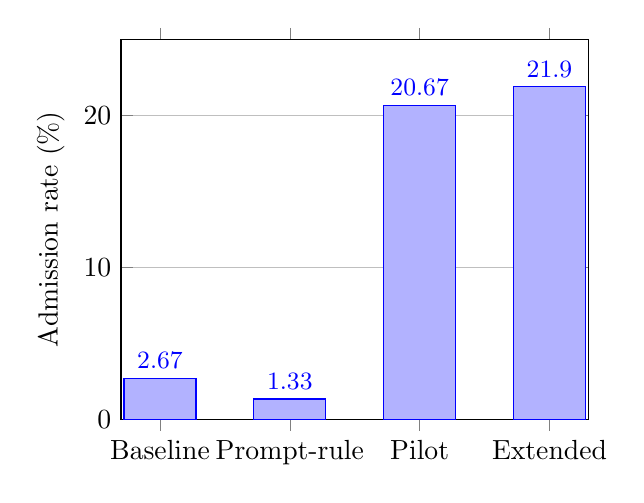
\begin{tikzpicture}
\begin{axis}[
  ybar, bar width=26pt,
  width=0.62\textwidth, height=6.4cm,
  symbolic x coords={Baseline, Prompt-rule, Pilot, Extended},
  xtick=data, ymin=0, ymax=25,
  ylabel={Admission rate (\%)},
  nodes near coords, every node near coord/.append style={font=\small},
  ymajorgrids=true,
]
\addplot coordinates {(Baseline,2.67) (Prompt-rule,1.33) (Pilot,20.67) (Extended,21.9)};
\end{axis}
\end{tikzpicture}
\caption{Admission rates by condition. The prompt-rule condition \emph{underperforms} the baseline; this is reported, not hidden, and motivated the copy-constrained redesign that produced the pilot and extended rows.}
\label{fig:gates}
\end{figure}

The gate runs inside a five-stage delivery pipeline, each stage producing its own receipt (Figure~\ref{fig:deploypipe}); the admit stage is the one that fails closed.

\begin{figure}[htbp]
\centering
\begin{tikzpicture}[
  node distance=0.9cm,
  box/.style={draw=black!70, rounded corners=3pt, align=center, font=\small, minimum width=2.2cm, minimum height=0.9cm},
  arr/.style={-{Stealth[length=3mm]}, thick}
]
\node[box] (d) {deploy};
\node[box, right=of d] (s) {source-bind};
\node[box, right=of s] (a) {attest};
\node[box, right=of a] (l) {live-verify};
\node[box, right=of l] (m) {admit};
\draw[arr] (d) -- (s);
\draw[arr] (s) -- (a);
\draw[arr] (a) -- (l);
\draw[arr] (l) -- (m);
\node[draw=none, font=\scriptsize, below=0.2cm of m] {bracket readback; fails closed};
\end{tikzpicture}
\caption{The delivery pipeline's five stages. The admit stage requires the runtime identity bracket (before==after) and sanitizes bracket violations to a handoff-unavailable error; the race case study is in Section~\ref{sec:edge}.}
\label{fig:deploypipe}
\end{figure}

\paragraph{What the gate measures.} An \emph{admitted} item is a derivation the teacher reproduces that satisfies the gate's admissibility predicate --- not a correctness score of the model in general. The design deliberately separates three things that a naive evaluation conflates: the corpus (fixed population 150, drawn from \texttt{doctrine-corpus-v2}), the instrument (the gate pinned at \texttt{ab0f1dd0}, teacher \texttt{SZL-Nemotron-Mini-4B-Estate-v1}), and the condition (the only variable between rows of Table~\ref{tab:gates}). Because only the condition varies, the four rates are comparable; because the population and instrument are pinned, a later re-run can only contradict the receipts, not quietly redefine them.

\paragraph{Honest disclosure of unlogged parameters.} The invocation arguments of the gate runs were not logged; the runs are bound to pinned defaults (seed 3407, temperature 0.7, max new tokens 512), recorded as the basis of the series rather than reconstructed after the fact. Condition-to-config mapping is fixed by the committed README and run-sequence timestamps. The series receipts are bound to the run archives at \texttt{frontier-54-runs} commit \texttt{3e5587156b1296d86f48c2fdb5facc24228747cb} and the \texttt{szl-forge} pipeline blob \texttt{06ae4de213bc3a99c00b1f7ac8400995d3a53c53} at commit \texttt{e5ceda6fa286843201a0665c0d97848e69c38b34}.

\paragraph{The negative result matters.} The prompt-rule condition (1.33\%) \emph{underperforms} the instruction-free baseline (2.67\%). A results-first publication would drop the losing condition; the estate's ledger keeps it, because the copy-constrained redesign that later reaches 20.67\% is only interpretable against the condition that failed. Negative conditions with published denominators are the estate's mechanism for making redesign decisions auditable.

\section{Incident Disclosure: The November 14 Card-Stamping Incident}
\label{sec:incident}

On November 14, 2026, 02:53--02:57 UTC, an off-route marketing-stamping job overwrote \textbf{138 public model cards} on the Hugging Face organization with a uniform fabricated template: identical model-index blocks, identical QLoRA training tables, uniform receipt badges, and uniform battery scores, applied regardless of whether the underlying repository possessed any such evidence (Hub commits \texttt{a2b1e8df} and \texttt{1c7d1590}, overwriting the correct publisher commit \texttt{1a7de2b2} 97 minutes after it landed). Under the estate's fail-closed doctrine the stamped cards were unverifiable per-model claims: an integrity incident, not a cosmetic one.

\subsection{Repair}
The repair pass was executed owner-authorized on the same day, with every action commit-addressed and read back:
\begin{itemize}
\item \textbf{101 byte-exact restorations} from the audited November 13 revisions (content-addressed digests, parent-commit and SHA-256 readback): \textbf{99} verdict \texttt{RESTORED}; \textbf{2} verdict \texttt{CARD\_REMOVED} (repositories whose audited state had no card at all --- the stamp had fabricated one, and the restore removed it back to audited absence). Zero errors. Per-repo log: \texttt{restore101\_log.jsonl}.
\item \textbf{31 honest-minimal rewrites} for repositories whose \emph{first} card was the stamp (the wave-4 trained set, created hours before the incident with no pre-stamp card): each rewritten card carries only per-repo facts (creation date via Hub API, exact base model and LoRA rank/alpha from \texttt{adapter\_config.json}, observed file list), an explicit \textbf{NOT MEASURED} section, a statement that no training receipt was published with the artifact, no invented license, a \texttt{publication\_eligible: false} flag, and a card-history note naming the off-route stamp. Per-repo log: \texttt{honest31\_log.jsonl}.
\end{itemize}
We report the disposition classes exactly as logged and do not smooth them into the incident total; the difference between the 138 overwritten cards and the dispositioned classes is itself part of the incident record.

\subsection{The license-pin follow-up: a second lesson, receipted}
The repair produced a second-order incident that is worth its own record because it changed procedure. The two \texttt{CARD\_REMOVED} repositories (\texttt{szl-lambda-gate}, \texttt{SZL-Forge-1.5B-ReceiptAgent}) had carried Apache-2.0 license metadata in their Hub tags; removing the stamped card also removed the tag, and the portfolio catalog --- which pins license metadata --- went red. The closure inputs showed both repositories had Apache-2.0 observed at audit, so the correct fix was not to argue with the catalog but to write honest cards restoring the evidenced license (both repositories carry Apache-2.0 \texttt{LICENSE} files in-tree). The fix landed as commits \texttt{2615fb7c} (an honest kernel card) and \texttt{dd5de54c} (a receipt-bound card for \texttt{SZL-Forge-1.5B-ReceiptAgent}, citing \texttt{training\_receipt.signed.json}, \texttt{eval\_receipt.signed.json}, and \texttt{owner\_pubkey.json} with SHA-256 digests; the receipts record base model Qwen2.5-1.5B-Instruct, final train loss 0.1038, evaluation 5/5, adversarial 6/6, signing key fingerprint \texttt{e7f01810aaa97394}). This is the estate's model of a \emph{receipt-bound card}: every measured number in it names the signed artifact that carries it.

\subsection{Root cause and lessons}
Transcript forensics traced the stamping writer to a prior agent session executing a blanket card-beautification campaign driven by an instruction of the form \emph{make all cards cutting-edge}. Three standing lessons are now doctrine:
\begin{enumerate}
\item \textbf{Never accept blanket card-beautification campaigns}; only per-model, receipt-bound upgrades. The honest-minimal card is the correct end state when evidence is absent.
\item \textbf{Card removal changes Hub metadata tags}: removing a stamped card also removed the Apache-2.0 license metadata the portfolio catalog pinned, reddening a downstream CI check. The fix (honest cards restoring the evidenced license) landed as commits \texttt{2615fb7c} and \texttt{dd5de54c}. Catalog license pins must be checked before any \texttt{CARD\_REMOVED} verdict.
\item \textbf{Uniformity is a stamp signature}: after convergence, an identical model-index + metrics + training-table signature across unrelated repositories is the re-stamp detector; honest cards are individually shaped by their evidence.
\end{enumerate}
The incident is disclosed here at full length precisely because the estate's central claim is trustworthiness, and trustworthiness is only demonstrable by publishing the failure, the repair, and the changed procedure.
